\externaldocument{chapter1}
\externaldocument{chapter5}
\chapter{Experiments and Results} % Main chapter title

\label{Chapter4} % For referencing the chapter elsewhere, use\ref{Chapter2} 

Performance of features from Convolution Neural Network are analysed in this chapter. To analyse CNNs, the datasets, evaluation metrics and network settings have to be fixed. In section \ref{dataset}, the details of source and target dataset are presented. In section \ref{evaluation}, the evaluation metrics that will be used are discussed. In section \ref{experiments}, experiments to analyse transfer learning on models selected in chapter 3, section \ref{model} are performed.

\section{Dataset}
\label{dataset}
More specific to our task than representing audio is finding a proper dataset of labelled pairs. To analyse \textit{transfer learning}, a large dataset is needed for the \textit{source task}. Popularly used \textit{Million Song Dataset} (MSD) \cite{MSD} contains a cluster of complimentary datasets, most of them annotated with \textit{social tags}. For instance, \textit{Last.fm} which forms a part of MSD contains annotations from users of an online radio application. But such social tags contribute to the \textit{audio-semantic} noise which we want to eliminate. The dataset that is mostly used for evaluating content-based algorithms is \textit{Magna Tag A Tune} dataset \cite{MTT}, where annotations are gathered through a game application that attracts users who are familiar with technical terms related to music. Hence the tags in this dataset are usually clean. Hence this would be a decent choice for our \textit{source task}.

\subsection{Dataset for source task}
\label{source}
The MagnaTagATune(MTT) dataset consists of 25,856 clips of 29.1-s mp3 files with 188 tags. These annotations are gathered from an online game called \textit{Tag a Tune}. A player is partnered up with another random player who cannot be communicated. Both listen to some track, and have to select appropriate tags. Then the players are asked one simple question : "Are we listening to same song?". Answering this correctly will earn them points. Frequently matched tags are collected to build a labelled dataset. This dataset is the largest available that comes close to minimizing the \textit{audio-semantic} noise. Only the top-50 tags from MTT are used for source task training. This is because, the CNN architecture in \cite{choi_cnn} for our analyses was also trained with top 50 tags (These tags were from MSD dataset. However, only the number '50' is important, which would otherwise change the size of final layer in neural network and might destroy the richness of pre-trained features). Since our target task is to approximate features for songs of arbitrary length, clips from same songs in MTT dataset are merged as a single sample.    

\subsection{Dataset for target task}
\label{target}
The annotations were gathered with one of the most straightforward approach - ask someone to listen to songs and tag them. This was done to have a clean mapping of perceptual properties to semantics. 842 songs approximately 5 - 8 min long , tagged by my supervisor Prof. Paolo Bientinesi in association with Prof. Marco Aluno (Professor of Composition and Theory at University EAFIT, Columbia) were used. Out of 842 songs, 100 are used for validation. The validation set is listed in appendix \ref{validationset}. 63 tags listed in appendix \ref{validationtags} were used for validation. 

\section{Evaluation}
\label{evaluation}
For multi-label classification with L labels, the performance of L binary classifiers are computed and averaged. Each label can belong to one of the class - \textit{positive} (1) or \textit{negative} (0). Area under Receiver operating characteristic Curve (AUC) is computed for each label. Mean of AUCs weighted by number of occurrence of each tag is reported. In this section, the need for this performance measure is discussed by comparing with other standard measures. To do this, some terminologies from information retrieval are recalled,\\
\\
\textbf{True Positives (TP) :} If the classifier admits a label as positive when the ground truth is also positive.\\
\textbf{True Negative (TN) :} If the classifier admits a label as negative when the ground truth is also negative.\\
\textbf{False Positives (FP) :} If the classifier admits a label as positive when the ground truth is negative.\\
\textbf{False Negative (FN) :} If the classifier admits a label as negative when the ground truth is positive.\\
\\
For a general tagging problem, most of the ground truth are \textit{negative} for most of the clips (That is, out of 900 songs, if 20 songs have the tag '\textit{electro}', then for this tag there are 20 \textit{ground truth positives} and 880 \textit{ground truth negatives}.\\
\\
\textbf{Accuracy :} To see why \textit{accuracy} will be an unfair measure, let us look at the definition of \textit{accuracy} for the label 'electro',
\[
  Accuracy = \frac{\sum TP + \sum TN}{900} = \frac{0+880}{900}
\]
Even if the classifier did not classify one 'electro' as positive, accuracy will be 0.98 with the contribution from 880 true negative samples.\\
\\
\textbf{Precision :} This does not tell anything about the percentage of false negatives. That is, even if the classifier \textit{correctly} admits one 'electro' as positive and 899 as negative (19 false negatives), \textit{precision} would be 1.0   
\[
  Precission = \frac{\sum TP}{\sum TP + \sum FP} = \frac{1}{1+0}
\]
\\
\textbf{Recall :} This is also not comprehensive because it does not tell anything about false positives. That is, even if the classifier admits 900 samples as positive (20 true positives and 880 false positives), \textit{recall} will be 1.0
\[
  Recall = \frac{\sum TP}{\sum TP + \sum FN} = \frac{20}{20+0} 
\]
\\
To strike a balance between \textit{recall} and \textit{precision}, the harmonic mean of both is often used, which is called \textit{F1} score. But to calculate all the metrics mentioned so far, some classifier threshold is required (That is, a binary classifier spits a number between 0 and 1 and if the number is above the threshold, the sample is classified as positive, otherwise negative). If the threshold is changed, then the performance can also change. To find a comprehensive measure for classifier performance, the metric should consider all threshold values.\\
\\ 
\textbf{Area under precision-recall curve :} When the\textit{ precision} and \textit{recall} are plotted for various threshold and the area under the precision-recall curve is found, the metric is termed as \textit{average precision}. Averaging the \textit{average precision} of L labels gives \textit{Mean average precision}.\\
\\
\textbf{Area under receiver operating characteristic curve (AUC) :} The \textit{fall-out} and \textit{recall} are plotted for various threshold and the area under the this curve is found. \textit{Fall-out} is defined as
\[
   Fall\_out = \frac{\sum FP}{\sum FP + \sum TN} 
\]
\textit{Recall} answers the question, 'when the ground truth of a sample is positive, how often does the classifier admits this sample as positive'. \textit{Fall-out} answers the question, 'when the ground truth of a sample is negative, how often does the classifier admits this sample as positive'. A random classifier would have an AUC of 0.5, meaning, for a binary random classification of an unknown sample there is 50\% chance for it to be true. Therefore, AUC can be thought of as a probability that a classifier would rank a randomly chosen observation with positive ground truth higher than a randomly chosen observation with negative ground truth. AUC is computed for L labels and averaged. Since the publications reviewed in previous chapter report this metric, we will also use the same. But in addition, we use \textit{weighted average} because our validation set is small and number of occurrences of each label is not balanced.\\
\\
Therefore, in all our experiments, \textit{Weighted averaged AUC} (WAUC) will be reported.

\section{Experiments}
\label{experiments}
 
As with any MIR task, the raw audio signal containing amplitude values in time domain is first down sampled and representation parameters are fixed (ref. \ref{stft}). The abstract algorithm for content based multi-label classifier is shown in algorithm \ref{exp:abstraction}. Function $R$ is the representation operation, $D$ represents dimensionality reduction operations (see Sec. \ref{dimension}), $T$ is the temporal approximation (see Sec. \ref{temporal}) and $C$ is the multi-label classifier (see Sec. \ref{classifier}). 
 
\begin{algorithm}
  \caption{$\textbf{pred}$ = $Model$($\textbf{a}$) }\label{exp:abstraction}
  \begin{algorithmic}[1]
    \Statex \textbf{Input :} $\textbf{a} \in \mathbb{R}^{N}$
    \Statex \textbf{Output :} $\textbf{pred}$ \Comment{indices of predicted labels}
    \State $\textbf{X} = R(\textbf{a})$ \Comment{$\textbf{X} \in \mathbb{R}^{R \times P}$}
    \State $\textbf{Y} = D(\textbf{X})$ \Comment{$\textbf{Y} \in \mathbb{R}^{T \times W}$}
    \State $\textbf{f} = T(\textbf{Y})$ \Comment{$\textbf{f} \in \mathbb{R}^{Z}$}
    \State $\bm{\zeta} = C(\textbf{f})$ \Comment{$\bm{\zeta} \in \mathbb{R}^{63}$}
    \State $\textbf{pred} = \{ b(\zeta_{i}) | b(\zeta_{i}) = 1 \}$ \Comment{$ i \in \{1,2,..,63\}, b( \zeta_{i}) \in \{0,1\}$}
  \end{algorithmic}
\end{algorithm}
\FloatBarrier

\subsection{Representation Parameters :}
\label{repPara}
As discussed in section \ref{model} of previous chapter, supervision is not imposed to compute representation operators. Hence, the following  representation parameters from \cite{choi_cnn} are fixed to compute \textit{log mel power spectrogram} for all experiments. 

\begin{table}[!htb]
\centering
\begin{tabular}{| p{.4\textwidth} | p{.3\textwidth}|}
\hline
\textbf{Parameter} & \textbf{Setting}\\
\hline
Sampling rate & 12 KHz\\
\hline
STFT window function & Hamming window\\
\hline
Size of each segment in STFT & 512 (42 ms)\\
\hline
Hop-Length & 256\\
\hline
FFT Size & 512\\
\hline
Mel bins & 96\\
\hline
\end{tabular}
\caption{Representation Parameters}\label{tab:repPara} 
\end{table}
\FloatBarrier

\noindent The function $R$ is thus replaced with log-mel power spectrogram computations. Step 1 - 4 in algorithm \ref{exp:a1} represents the computation of log mel-power spectrogram (see Chapter 2, Sec. \ref{mel}). The abstract algorithm for our experiments is shown below. FFT was computed using the python library \textit{Librosa}\cite{Librosa}. 
\begin{algorithm}
  \caption{$\textbf{pred}$ = $Model$($\textbf{a}$) }\label{exp:a1}
  \begin{algorithmic}[1]
    \Statex \textbf{Input :} $\textbf{a} \in \mathbb{R}^{12000.t}$
    \Statex \textbf{Output :} $\textbf{pred}$ \Comment{indices of predicted labels}
    \State $\textbf{C} = \textbf{a} \star {\textbf{W}_{STFT}}^{(256)}$ \Comment{$\textbf{C} \in \mathbb{R}^{512 \times P}, \textbf{W}_{STFT} \in \mathbb{R}^{512 \times 512}$}
    \State $\textbf{C} \leftarrow \textbf{C} \odot \textbf{C}$
    \State $\textbf{X} = \textbf{C} \star {\textbf{W}_{MEL}}^{(512)}$ \Comment{$\textbf{X} \in \mathbb{R}^{96 \times P}, \textbf{W}_{MEL} \in \mathbb{R}^{96 \times 512}$}
    \State $\textbf{X} \leftarrow ln(\textbf{X})$
    \State $\textbf{Y} = D(\textbf{X})$ \Comment{$\textbf{Y} \in \mathbb{R}^{T \times W}$}
    \State $\textbf{f} = T(\textbf{Y})$ \Comment{$\textbf{f} \in \mathbb{R}^{Z}$}
    \State $\bm{\zeta} = C(\textbf{f})$ \Comment{$\bm{\zeta} \in \mathbb{R}^{63}$}
    \State $\textbf{pred} = \{ b(\zeta_{i}) | b(\zeta_{i}) = 1 \}$ \Comment{$ i \in \{1,2,..,63\}, b( \zeta_{i}) \in \{0,1\}$}
  \end{algorithmic}
\end{algorithm}
\FloatBarrier

\subsection{Perceptron Settings}
\label{percentron_s}
Two layer perceptron (equation \ref{eq:mlp}) with rectified linear units activation ($ReLU$) activation in the hidden layer is used for classification $C$ (step 7 of algorithm \ref{exp:a2}). $ReLU$ is used to handle the vanishing gradient problem. The operators $\textbf{W}_{L1}$ and $\textbf{W}_{L2}$ are solved for optimality. (see Sec. \ref{training}). To find the optimal settings for perceptron, functions $D$ and $T$ are fixed. Thus, log mel-power spectrogram is reduced to MFCC features and approximated to a fixed size representation with Bag of Frames features. Hence, the error is back-propagated only to the classifier $C$ and the resulting learning problem is said to be shallow.  

\begin{algorithm}
\begin{minipage}{0.15\textwidth}
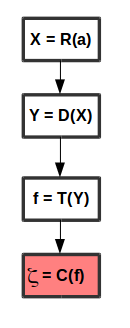
\includegraphics[width=0.75\textwidth]{ce1}
\end{minipage}
  \begin{minipage}{0.80\textwidth}
  \caption{$\textbf{pred}$ = $Model$($\textbf{a}$) }\label{exp:a2}
  \begin{algorithmic}[1]
    \Statex \textbf{Input :} $\textbf{a} \in \mathbb{R}^{12000.t}$
    \Statex \textbf{Output :} $\textbf{pred}$ \Comment{indices of predicted labels}
    \State $\textbf{C} = \textbf{a} \star {\textbf{W}_{STFT}}^{(256)}$ \Comment{$\textbf{C} \in \mathbb{R}^{512 \times P}, \textbf{W}_{STFT} \in \mathbb{R}^{512 \times 512}$}
    \State $\textbf{C} \leftarrow \textbf{C} \odot \textbf{C}$
    \State $\textbf{X} = \textbf{C} \star {\textbf{W}_{MEL}}^{(512)}$ \Comment{$\textbf{X} \in \mathbb{R}^{96 \times P}, \textbf{W}_{MEL} \in \mathbb{R}^{96 \times 512}$}
    \State $\textbf{X} \leftarrow ln(\textbf{X})$
    \State $\textbf{Y} = \textbf{X} \star {\textbf{W}_{MFCC}}^{(96)}$ \Comment{$\textbf{Y} \in  \mathbb{R}^{90 \times P}, \textbf{W}_{MFCC} \in \mathbb{R}^{90 \times 96}$}
    \State $\textbf{f} = BagOfFrames(\textbf{Y})$ \Comment{$\textbf{f} \in \mathbb{R}^{Z}$}
    \State $\bm{\zeta} = \sigma ({\color{red} \textbf{W}_{L2}} ReLU ({\color{red}\textbf{W}_{L1}}\textbf{f})) $ \Comment{$\bm{\zeta} \in \mathbb{R}^{63}, \textbf{W}_{L2} \in \mathbb{R}^{63 \times H}, \textbf{W}_{L1} \in \mathbb{R}^{H \times Z}$}
    \State $\textbf{pred} = \{ b(\zeta_{i}) | b(\zeta_{i}) = 1 \}$ \Comment{$ i \in \{1,2,..,63\}, b( \zeta_{i}) \in \{0,1\}$}
  \end{algorithmic}
  \end{minipage}
\end{algorithm}
\FloatBarrier

\noindent The network is trained with ADAM optimizer. The training settings that are used in this thesis were explained in Chapter 2, section \ref{training}. All ADAM parameters except the learning rate $\eta$ are used as proposed in  \cite{adam_o}. The learning rate can be different for different sections of the network and hence we differentiate the learning rate of the classifier with subscript $c$ ($\eta_{c}$). The learning rate is reduced by factor $\gamma_{c}$ every $step_{c}$ iterations. This is done because in the beginning, large learning rate is needed to approach the solution, but as the training approaches actual solution, learning rate has to be reduced. Otherwise, the solution might be sub optimal. However, the learning rate is not reduced below $1^{-6}$. Even though the classifier is shallow, the network is first trained on the MTT dataset (source task) until convergence. The resulting weights are used as initialization for training on target dataset. Since our aim is to analyse only the CNNs, the training hyper-parameters values for the classifier are fixed with values shown in table \ref{tab:a2}. Neural network modules from the framework \textit{Torch}\cite{Torch} were used for implementation and training. 

\begin{table}[!htb]
\centering
\begin{tabular}{| p{.3\textwidth} | p{.3\textwidth} | p{.3\textwidth} |}
\hline
\textbf{Hyper-parameter} & \textbf{Source task} & \textbf{Target task}\\
\hline
${\eta}_{c}$ & $1^{-2}$ & $1^{-3}$ \\ 
\hline
${\gamma}_{c}$ & $0.1$ & $ 0.1$\\
\hline
${step}_{c}$ & 10000 & 3000 \\
\hline
\end{tabular}
\caption{Training Hyper-Parameters for Classifier}\label{tab:a2} 
\end{table}
\FloatBarrier

\noindent To set up a two layer neural network, the size of the classifier input (or feature) $Z$, the dimension of hidden layer $H$ and the size of the output $L$ should be known. The size of the output is equal to the number of labels in test. 63 labels are used for validation in target set. The experiments for different $H$ and $Z$ and their resulting WAUC scores are shown in table \ref{tab:a3}. (Here the features size ($Z$) resulting from the Bag of frames is equal to the number of cluster centres to be chosen)
 
\begin{table}[!htb]
\centering
\begin{tabular}{| p{.24\textwidth} | p{.24\textwidth}| p{.24\textwidth}| p{.24\textwidth} |}
\hline
& $H = \textbf{512}$ & $H = \textbf{1024}$ & $H = \textbf{2048}$\\
\hline
$Z = \textbf{512}$  & 0.63 & 0.64 & 0.63\\
\hline
$Z = \textbf{1024}$ & 0.64 & \textbf{0.67 }& 0.62\\ 
\hline
$Z = \textbf{2048}$ & 0.61 & 0.61 & 0.59\\
\hline
\end{tabular}
\caption{Hyper parameter search : Classifier hidden dimension (H), Feature dimension (Z)}\label{tab:a3} 
\end{table}
\FloatBarrier

\noindent When the feature size is 512, it can be seen that the performance is capped around 0.64 for different hidden size. The performance improves with feature size 1024. However, the performance decreases when the dimension increases to 2048. This tells us that the classifier complexity with hidden size 512 is in-sufficient. But the model begins to over fit (learns the noisy data) when the size increases to 2048. Hence the feature dimension ($Z$) and hidden dimension ($H$) are fixed to \textbf{1024} for all the remaining analyses. 

\subsection{RNN Settings}
\label{rnn_s}
The error from classifier $C$ is back-propagated into the temporal approximation function $T$ with a 2 layer LSTM. Therefore, the Bag of frames algorithm is replaced with LSTM. The operators of LSTM $\bm{\Phi_{R1}}$ and $\bm{\Phi_{R2}}$ are solved to sequentially combine frame-wise features into a fixed size projection. The LSTM operators
\[
\bm{\Phi}_{Rj} = \{\textbf{W}_{(k,j)}, \textbf{U}_{(k,j)}\} \qquad k \in \{i,o,g,c\}, j \in \{1,2\}
\] 
were described in Chapter 2, section \ref{rnn}. Thus the learning is pushed into the temporal approximation function. While combining MFCC features, the number of STFT frames can be large for longer songs and the information at the beginning of sequence can get lost. To get around this problem, the first layer of LSTM is a \textit{sequence to one} network that combines frames up to 29.1s. The second layer of \textit{sequence to one} LSTM combines features from every 29.1s frame to a fixed sized projection. This computation is illustrated in step 6 - 12 of algorithm \ref{exp:a3}. There are 1366 STFT frames for 29.1s of 12 KHz sampled signal. Drop out with probability $p$ is used as the transition operation (referred in chapter 2, algorithm \ref{alg:2lstm}). Drop out acts as a regularizer that prevents the network from over-fitting.
\begin{algorithm}
\begin{minipage}{0.15\textwidth}
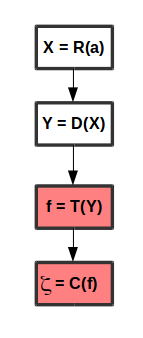
\includegraphics[width=0.75\textwidth]{ce2}
\end{minipage}
  \begin{minipage}{0.80\textwidth}
  \caption{$\textbf{pred}$ = $Model$($\textbf{a}$) }\label{exp:a3}
   {\fontsize{8}{0}
  \begin{algorithmic}[1]
    \Statex \textbf{Input :} $\textbf{a} \in \mathbb{R}^{12000.t}$
    \Statex \textbf{Output :} $\textbf{pred}$ \Comment{indices of predicted labels}
    \State $\textbf{C} = \textbf{a} \star {\textbf{W}_{STFT}}^{(256)}$ \Comment{$\textbf{C} \in \mathbb{R}^{512 \times P}, \textbf{W}_{STFT} \in \mathbb{R}^{512 \times 512}$}
    \State $\textbf{C} \leftarrow \textbf{C} \odot \textbf{C}$
    \State $\textbf{X} = \textbf{C} \star {\textbf{W}_{MEL}}^{(512)}$ \Comment{$\textbf{X} \in \mathbb{R}^{96 \times P}, \textbf{W}_{MEL} \in \mathbb{R}^{96 \times 512}$}
    \State $\textbf{X} \leftarrow ln(\textbf{X})$
    \State $F = 1366$
    \State $W = floor(\frac{P}{F})$
    \For{$i \in \{0,..,W\}$}
      \State $ \textbf{G} \leftarrow \textbf{X}[:,(i+1)F]$
      \State $\textbf{Y} \leftarrow \textbf{G} \star {\textbf{W}_{MFCC}}^{(96)}$ \Comment{$\textbf{Y} \in \mathbb{R}^{90 \times F}, \textbf{W}_{MFCC} \in \mathbb{R}^{90 \times 96}$}
      \State $\textbf{F}[i] = {Drop}_{(p)}(Seq2One\_LSTM(\textbf{Y} | {\color{red}\bm{\Phi}_{R2}} ))$ \Comment{$\textbf{F} \in \mathbb{R}^{T \times W}$}
    \EndFor
    \State $\textbf{f} = {Drop}_{(p)}(Seq2One\_LSTM(\textbf{F} | {\color{red}\bm{\Phi}_{R1}}))$ \Comment{$\textbf{f} \in \mathbb{R}^{1024}$}
    \State $\bm{\zeta} = \sigma ({\color{red} \textbf{W}_{L2}} ReLU ({\color{red}\textbf{W}_{L1}}\textbf{f})) $ \Comment{$\bm{\zeta} \in \mathbb{R}^{63}, \textbf{W}_{L2} \in \mathbb{R}^{63 \times 1024}, \textbf{W}_{L1} \in \mathbb{R}^{1024 \times 1024}$}
    \State $\textbf{pred} = \{ b(\zeta_{i}) | b(\zeta_{i}) = 1 \}$ \Comment{$ i \in \{1,2,..,63\}, b( \zeta_{i}) \in \{0,1\}$}
  \end{algorithmic}
  }
  \end{minipage}
\end{algorithm}
\FloatBarrier

\noindent To set up a 2 layer LSTM, the size of hidden projection $T$ and the drop-out probability $p$ have to be known. Training settings for source and target tasks are same as that of the classifier. WAUC scores for different  $p$ and $T$ are shown in table \ref{tabl:a4}.
\begin{table}[!htb]
\centering
\begin{tabular}{| p{.24\textwidth} | p{.24\textwidth}| p{.24\textwidth}| p{.24\textwidth} |}
\hline
& $T = \textbf{512}$ & $T = \textbf{1024}$ & $T = \textbf{2048}$\\
\hline
$p = \textbf{0}$  & 0.66 & 0.61 & 0.59\\
\hline
$p = \textbf{0.3}$ & 0.68 & \textbf{0.74} & 0.68\\ 
\hline
$p = \textbf{0.5}$ & 0.67 & 0.71 & 0.64\\
\hline
\end{tabular}
\caption{Hyper parameter search : RNN hidden dimension (T), Drop-out probability (p)}\label{tabl:a4} 
\end{table}
\FloatBarrier

\noindent The optimum classifier settings from experiments in previous section is used ($H = Z = 1024$). The hidden dimension ($T$) 1024 is found to be optimal. It can be seen that the network over-fits without the drop-out ($p = 0$). Therefore, $p = 0.3$ and $T = 1024$ is used fixed for remaining analyses.

\subsubsection{Black-box LSTM}
\begin{minipage}{0.15\textwidth}
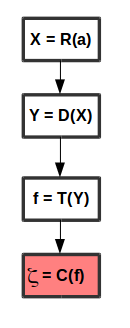
\includegraphics[width=0.75\textwidth]{ce1}
\end{minipage}
\begin{minipage}{0.80\textwidth}
The operators of LSTM trained on the source task can also be used as black-box feature extractor for the target task (that is, LSTM is not further trained with target data). This is done because fine-tuning on the target training set might degrade the operators sometimes. This could either be because of convergence of source task training towards general purpose features or because of in-sufficient training data in the target set. To check this, LSTM trained on the source dataset is used as a black-box feature extractor for the target task. But, for the optimal LSTM settings from experiments in previous section ($p = 0.3$, $T=1024$), WAUC drops to \textbf{0.65}. This shows that the source task features cannot be used as general purpose features and still needs task-dependent training. 
\end{minipage}

\subsection{Analyses of CNN}
\label{cnn_s}
With the percepton and RNN settings from section \ref{percentron_s} and \ref{rnn_s}, we are now ready to analyse CNNs. Instead of MFCC feature extraction operators ($\textbf{W}_{MFCC}$), hierarchical layers of learn-able operators $\bm{\Phi}_{C}$ are used (see Sec. \ref{stacked}). As discussed in chapter 3, section \ref{fe1}, 5 layers of 2D convolution neural network architecture from \cite{choi_cnn} is used (see algorithm \ref{alg:choicnn}). Thus,
\[
\bm{\Phi}_{C} = \{\textbf{W}_{Cj}\} \qquad j \in \{1,2,3,4,5\}
\]    
Features are extracted with CNN over 29.1s log mel-spectrogram. The resulting features from every 29.1s frames are sequentially combined to a fixed size representation with LSTM. (In algorithm \ref{exp:a3}, the input to first layer of RNN was features from every STFT frame. But now, the input is from every 29.1s frame, and this sequence is not as large as the former). Two layers of LSTM with \textit{sequence to sequence} layer in between is used (see algorithm \ref{alg:2lstm}).  
\begin{algorithm}
\begin{minipage}{0.15\textwidth}
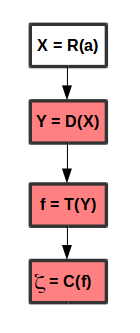
\includegraphics[width=0.75\textwidth]{ce3}
\end{minipage}
  \begin{minipage}{0.80\textwidth}
  \caption{$\textbf{pred}$ = $Model$($\textbf{a}$) }\label{exp:a4}
   {\fontsize{8}{0}
  \begin{algorithmic}[1]
    \Statex \textbf{Input :} $\textbf{a} \in \mathbb{R}^{12000.t}$
    \Statex \textbf{Output :} $\textbf{pred}$ \Comment{indices of predicted labels}
    \State $\textbf{C} = \textbf{a} \star {\textbf{W}_{STFT}}^{(256)}$ \Comment{$\textbf{C} \in \mathbb{R}^{512 \times P}, \textbf{W}_{STFT} \in \mathbb{R}^{512 \times 512}$}
    \State $\textbf{C} \leftarrow \textbf{C} \odot \textbf{C}$
    \State $\textbf{X} = \textbf{C} \star {\textbf{W}_{MEL}}^{(512)}$ \Comment{$\textbf{X} \in \mathbb{R}^{96 \times P}, \textbf{W}_{MEL} \in \mathbb{R}^{96 \times 512}$}
    \State $\textbf{X} \leftarrow ln(\textbf{X})$
    \State $F = 1366$
    \State $W = floor(\frac{P}{F})$
    \For{$i \in \{0,..,W\}$}
      \State $ \textbf{G} \leftarrow \textbf{X}[:,(i+1)F]$
      \State $\textbf{Y}[i] = CHOI\_CNN(\textbf{G} | {\color{red} \bm{\Phi}_{C}})$ \Comment{$\textbf{Y} \in \mathbb{R}^{1024 \times W}$}
     \EndFor
     \State $\textbf{F} = {Drop}_{(0.3)}(Seq2Seq\_LSTM(\textbf{Y} | {\color{red}\bm{\Phi}_{R2}} ))$ \Comment{$\textbf{F} \in \mathbb{R}^{1024 \times W}$}
    \State $\textbf{f} = {Drop}_{(0.3)}(Seq2One\_LSTM(\textbf{F} | {\color{red}\bm{\Phi}_{R1}}))$ \Comment{$\textbf{f} \in \mathbb{R}^{1024}$}
    \State $\bm{\zeta} = \sigma ({\color{red} \textbf{W}_{L2}} ReLU ({\color{red}\textbf{W}_{L1}}\textbf{f})) $ \Comment{$\bm{\zeta} \in \mathbb{R}^{63}, \textbf{W}_{L2} \in \mathbb{R}^{63 \times 1024}, \textbf{W}_{L1} \in \mathbb{R}^{1024 \times 1024}$}
    \State $\textbf{pred} = \{ b(\zeta_{i}) | b(\zeta_{i}) = 1 \}$ \Comment{$ i \in \{1,2,..,63\}, b( \zeta_{i}) \in \{0,1\}$}
  \end{algorithmic}
  }
  \end{minipage}
\end{algorithm}
\FloatBarrier

\subsubsection{Source task training}

\noindent The CNN architecture that we use has been already analysed in \cite{choi_cnn} for multi-label classification task with fixed sized input on MSD dataset. These weights are used as initialization for training our source task model that handles input of arbitrary size. The CNN hyper parameters (number of layers, transition functions, filter sizes and number of filters in each layer) proposed in \cite{choi_cnn} is used. But we search for optimum training parameters for CNN ($\eta_{c}, step_{c}$). The reduction factor $\gamma_{c}$ is fixed at 0.1. $\eta_{c}$ and $step_{c}$ can be different for different CNN layers. However, the CNN is split into two sections : layer 1,2 and layer 3,4,5. The training hyper-parameters are set separately for each section. Table \ref{tab:a5} shows WAUC of experiments on source set where only the last three out of five layers of CNN is fine-tuned. That is, the learning rate for the first two layers is 0 (Freeze).    
\begin{table}[!htb]
\centering
\begin{tabular}{| p{.40\textwidth} | p{.40\textwidth}| p{.15\textwidth}| }
\hline
$\textbf{Layer = 1,2}$ & $\textbf{Layer = 3,4,5}$ & \textbf{WAUC}\\
\hline
Freeze & $(1^{-3}; 30K)$ & 0.79\\
\hline
Freeze & $(1^{-3}; 50K)$ & \textbf{0.81}\\
\hline
Freeze & $(1^{-3}; 70K)$ & 0.74\\
\hline
Freeze & $(1^{-4}; 30K)$ & 0.79\\
\hline
Freeze & $(1^{-4}; 50K)$ & \textbf{0.81}\\
\hline
Freeze & $(1^{-4}; 70K)$ & 0.77\\
\hline
\end{tabular}
\caption{Source task experiments with 1st two layers freezed : $(\eta_{f}, {step}_{f})$}\label{tab:a5} 
\end{table}
\FloatBarrier
\noindent It can be seen that learning rate $1^{-3}$ and $1^{-4}$ stepping down every 50K iterations have similar performance. In table \ref{tab:a6}, WAUC of experiments where the whole CNN is trained are reported. The learning rate and step down for the last three layers are chosen from the experiments in table \ref{tab:a5}.  
\begin{table}[!htb]
\centering
\begin{tabular}{| p{.40\textwidth} | p{.40\textwidth}| p{.15\textwidth}| }
\hline
$\textbf{Layer = 1,2}$ & $\textbf{Layer = 3,4,5}$ & \textbf{WAUC}\\
\hline
$(1^{-5}; 50K)$ & $(1^{-3}; 50K)$ & 0.82\\
\hline
$(1^{-5}; 50K)$ & $(1^{-4}; 50K)$ & 0.79\\
\hline
$(1^{-4}; 50K)$ & $(1^{-3}; 50K)$ & \textbf{0.84}\\
\hline
$(1^{-4}; 50K)$ & $(1^{-4}; 50K)$ & 0.77\\
\hline
$(1^{-4}; 70K)$ & $(1^{-3}; 50K)$ & 0.82\\
\hline
$(1^{-4}; 70K)$ & $(1^{-4}; 50K)$ & 0.79\\
\hline
$(1^{-3}; 50K)$ & $(1^{-3}; 50K)$ & 0.83\\
\hline
$(1^{-3}; 50K)$ & $(1^{-4}; 50K)$ & 0.76\\
\hline
$(1^{-3}; 70K)$ & $(1^{-3}; 50K)$ & 0.81\\
\hline
$(1^{-3}; 70K)$ & $(1^{-4}; 50K)$ & 0.76\\
\hline
\end{tabular}
\caption{Source task experiments with all layers trained : $(\eta_{f}, {step}_{f})$}\label{tab:a6}
\end{table}
\FloatBarrier
\noindent Training all the layers of CNN on the source dataset with learning rate $1^{-4}$ in layers 1,2 and $1^{-3}$ in layers 3,4,5 is shown to be optimal. It can also be inferred that the last layers of CNN tend to find task specific features not suited for general purpose classification. 
 
\subsubsection{Target task training}
After the training converges on the source dataset, the weights are initialized for training on target dataset. The training hyper-parameters can be different for the target task. The step down iteration is lower for the target task because of smaller training data. 
\begin{table}[!htb]
\centering
\begin{tabular}{| p{.40\textwidth} | p{.40\textwidth}| p{.15\textwidth}| }
\hline
$\textbf{Layer = 1,2}$ & $\textbf{Layer = 3,4,5}$ & \textbf{WAUC}\\
\hline
Freeze & $(1^{-3}; 5K)$ & 0.65\\
\hline
Freeze & $(1^{-3}; 10K)$ & 0.63\\
\hline
Freeze & $(1^{-3}; 20K)$ & 0.61\\
\hline
Freeze & $(1^{-4}; 5K)$ & 0.67\\
\hline
Freeze & $(1^{-4}; 10K)$ & \textbf{0.68}\\
\hline
Freeze & $(1^{-4}; 20K)$ & 0.63\\
\hline
\end{tabular}
\caption{Target task experiments with 1st two layers freezed : $(\eta_{f}, {step}_{f})$}\label{tab:a7} 
\end{table}

\begin{table}[!htb]
\centering
\begin{tabular}{| p{.40\textwidth} | p{.40\textwidth}| p{.15\textwidth}| }
\hline
$\textbf{Layer = 1,2}$ & $\textbf{Layer = 3,4,5}$ & \textbf{WAUC}\\
\hline
$(1^{-6}; NA)$ & $(1^{-4}; 10K)$ & 0.64\\
\hline
$(1^{-5}; 10K)$ & $(1^{-4}; 10K)$ & \textbf{0.71}\\
\hline
$(1^{-5}; 20K)$ & $(1^{-4}; 10K)$ & 0.69\\
\hline
$(1^{-4}; 10K)$ & $(1^{-4}; 10K)$ & 0.68\\
\hline
$(1^{-4}; 20K)$ & $(1^{-4}; 10K)$ & 0.67\\
\hline
\end{tabular}
\caption{Target task experiments with all layers trained : $(\eta_{f}, {step}_{f})$}\label{tab:a8}
\end{table}
\FloatBarrier
\noindent Fine-tuning all the layers of CNN on the target dataset with learning rate $1^{-5}$ in layers 1,2 and $1^{-4}$ in layers 3,4,5 is shown to be optimal. Individual performance of every label in validation is shown in appendix \ref{tagperformance}. However, the performance is slightly lesser than what is achieved with MFCC features.

\subsubsection{Black-box CNN + Fine-tune LSTM}  
\begin{minipage}{0.15\textwidth}
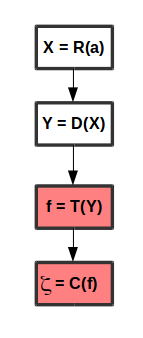
\includegraphics[width=0.75\textwidth]{ce2}
\end{minipage}
\begin{minipage}{0.80\textwidth}
To see if the reduction in performance is because of fine-tuning on a small target dataset, CNN trained on source data is used as black-box feature extractor for target task (CNN is not trained on target data). This tells us if the features of CNN trained on source task are richer than MFCCs. The LSTM is however fine tuned with the settings discussed earlier. But WAUC drops to \textbf{0.65}, which shows that the CNN features from source task may not be rich enough. However, it is still not clear because we do not know if fine-tuning LSTM on target data is optimal for extracting information from CNN features. 
\end{minipage}

\subsubsection{Black-box CNN + Black-box LSTM}
\begin{minipage}{0.15\textwidth}
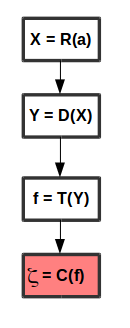
\includegraphics[width=0.75\textwidth]{ce1}
\end{minipage}
\begin{minipage}{0.80\textwidth}
Now both CNN and LSTM are used as black-box feature extractor. Thus, only the classifier is trained on target data. The WAUC further drops to \textbf{0.63}. It can be seen that training (source data) both CNN and LSTM in a single pipeline restricts the optimality of RNN (Recall that MFCC + LSTM performed better than MFCC + BoF). This could result in CNN features that are not as rich as MFCC. 
\end{minipage}

\subsubsection{Black-box CNN + Bag of Frames}
\begin{minipage}{0.15\textwidth}
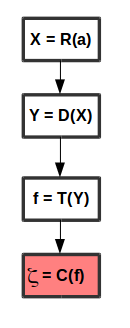
\includegraphics[width=0.75\textwidth]{ce1}
\end{minipage}
\begin{minipage}{0.80\textwidth}
Replacing black-box LSTM with Bag of frames algorithm for black-box CNN features, WAUC increases to \textbf{0.67}. Thus, CNN features obtained by training CNN + LSTM on the source task data still contain information for classification. But, CNN features are not as rich as MFCC for our target task.
\end{minipage}

\section{Summary of results}
\label{results}
Transfer learning with CNN and LSTM for music tagging task were analysed by stage-wise induction of supervised learning deeper into the model. Classification on MFCC features approximated with Bag of frames algorithm does not require supervised learning and hence used as baseline for comparison. LSTM were used to introduce supervised learning of temporal approximation function. CNN and LSTM were then trained in a single pipeline to introduce supervision into reduction operations. Performances of features resulting from LSTM and CNN with and without (black-box) fine-tuning on target data have been discussed. 

\subsubsection{Analyses of LSTM}
LSTM analyses are summarized in table \ref{tab:a9}. LSTM trained on source task, but used as a black box extractor on target task performs below the BoF baseline. But when LSTM is fine-tuned on target data, performance improves significantly. Therefore, it is seen that LSTM is still not sufficient to realize general purpose approximation operators, but requires task dependent fine-tuning to out-perform BoF.   

\begin{table}[!htb]
\centering
   \begin{tabular}{ | p{0.7\textwidth} | p{0.2\textwidth} |}
    \hline
    \textbf{Model} & \textbf{WAUC} \\ \hline
    MFCC + BoF &  0.67\\ \hline
    MFCC + Black-box LSTM &  0.65 \\ \hline
    MFCC + Fine-tune LSTM  &  \textbf{0.74}\\ \hline
    \hline
    \end{tabular}
    \caption{Summary of LSTM analyses}\label{tab:a9}
\end{table}
\FloatBarrier

\subsubsection{Analyses of CNN}
CNN analyses are summarized in table \ref{tab:a10}. CNN and LSTM were trained in a single pipeline on the source dataset. Performance of black-box CNN with Bag of frames approximation is again better than black-box LSTM. But performance of black-box CNN with fine-tuned LSTM is lesser than it's MFCC counter-part and this shows that CNN features are not as rich as MFCC to serve as general purpose feature extractor. Fine-tuning CNN improves the performance, but it is still slightly lesser than MFCC. This shows that fine-tuning CNN on smaller dataset still cannot outperform MFCC for our target task.
  
\begin{table}[!htb]
\centering
   \begin{tabular}{ | p{0.7\textwidth} | p{0.2\textwidth} |}
    \hline
    \textbf{Model} & \textbf{WAUC} \\ \hline
    Black-box CNN + BoF & 0.67 \\ \hline 
    Black-box CNN + Black-box LSTM & 0.63 \\ \hline 
    Black-box CNN + Fine-tune LSTM & 0.65 \\ \hline
    Fine-tune CNN + Fine-tune LSTM &  0.71 \\ \hline
    \hline
    \end{tabular}
    \caption{Summary of CNN + LSTM analyses}\label{tab:a10}
\end{table}
\FloatBarrier
\noindent The training\footnote{https://github.com/as641651/CNNs-for-automatic-tagging-of-music-tracks} and run-time\footnote{https://github.com/as641651/RythmCap} codes are available in separate git repositories



